% background.tex

\chapter{Background}

%The free energy difference between the bound and unbound states of a protein-ligand system ($\Delta G_{bind}$) provides insight into the likelihood of the binding reaction. Furthermore, the difference between the $\Delta G_{bind}$ of two different protein-ligand pairs (their $\Delta \Delta G$) informs which pair binds better to each other.

\section{Free energy calculations}

Biological systems of fixed connectivity can be represented as a set of conformations that are defined by a molecular topology, with varying bond lengths, bond angles, torsional angles and atomic positions\cite{shirts2007alchemical,christ2010basic,pohorille2010good}. In the canonical ensemble, these conformations are Boltzmann distributed, meaning they follow the distribution $p(\boldsymbol{x})=\exp(-\beta U(\boldsymbol{x})) / Z$, where $\beta$ is the inverse temperature of the system, $\boldsymbol{x}$ represents a conformation, $U(\boldsymbol{x})$ represents the potential energy of a conformation $\boldsymbol{x}$, and $Z$ represents the partition function, defined as $Z=\int_\Omega \exp(-\beta U(\boldsymbol{x})) d\boldsymbol{x}$, where $\Omega$ represents the complete set of conformations. Hereafter, the terms partition function and normalizing constant will be used interchangeably, and $\exp(-\beta U(\boldsymbol{x}))$ will be referred to as the Boltzmann weight, unnormalized density or $q(\boldsymbol{x})$.

The free energy of a system is given by $G=-\beta^{-1} \log(Z)$, and the free energy difference between two systems is given by: 
\begin{equation}\label{freeeneqn} 
\Delta G_{1\rightarrow2} = -\beta^{-1} \log(Z_2/Z_1)
\end{equation} 

\noindent These systems are frequently selected to define the bound and unbound states of a protein-ligand pair, making the free energy difference a $\Delta G_{bind}$, which is representative of the likelihood of the binding reaction. Furthermore, the difference between the $\Delta G_{bind}$ of two different protein-ligand pairs (their $\Delta \Delta G$) informs which pair binds better to each other.
Computational prediction of $\Delta \Delta G$ for minor ligand modifications could significantly speed up lead optimization steps in a drug development context, by focusing the search on promising modifications selected by a simulation-based prescreening step.

For biological systems of interest, namely those describing interactions between a macromolecule and a small molecule or protein ligand, the partition function is unfeasible to calculate directly due to the size of the conformation space and the impossibility of writing out the partition function analytically\cite{christ2010basic}. The goal of a free energy calculation is to estimate partition functions, or more commonly, ratios thereof.

Free energy calculations involve two components\cite{shirts2007alchemical,christ2010basic}: conformational sampling and estimation. Because the distributions of macromolecules are complex, multimodal and high dimensional\cite{shirts2007alchemical,christ2010basic}, with large regions of low density, sampling requires specialized methods. The most widely used method for conformational sampling is molecular dynamics (MD)\cite{christ2010basic}, which generates conformations by simulating the time varying movement of a macromolecule by numerical integration of the equations of motion. For large macromolecular systems, this is a very computationally costly process. With typical current computational resources, the \si{\micro\second} time scale is the current limit of timescales accessible via MD\cite{vandivort2008long,salomon2013routine}. Relevant biological movements for macromolecules such as allosteric modulation and molecular recognition are thought to occur on the \si{\micro\second} to \si{\milli\second} time scale\cite{harvey2012high}. This disparity means that direct simulation of binding events and calculation of $\Delta G_{bind}$ is impossible. 

\begin{figure}
\centering
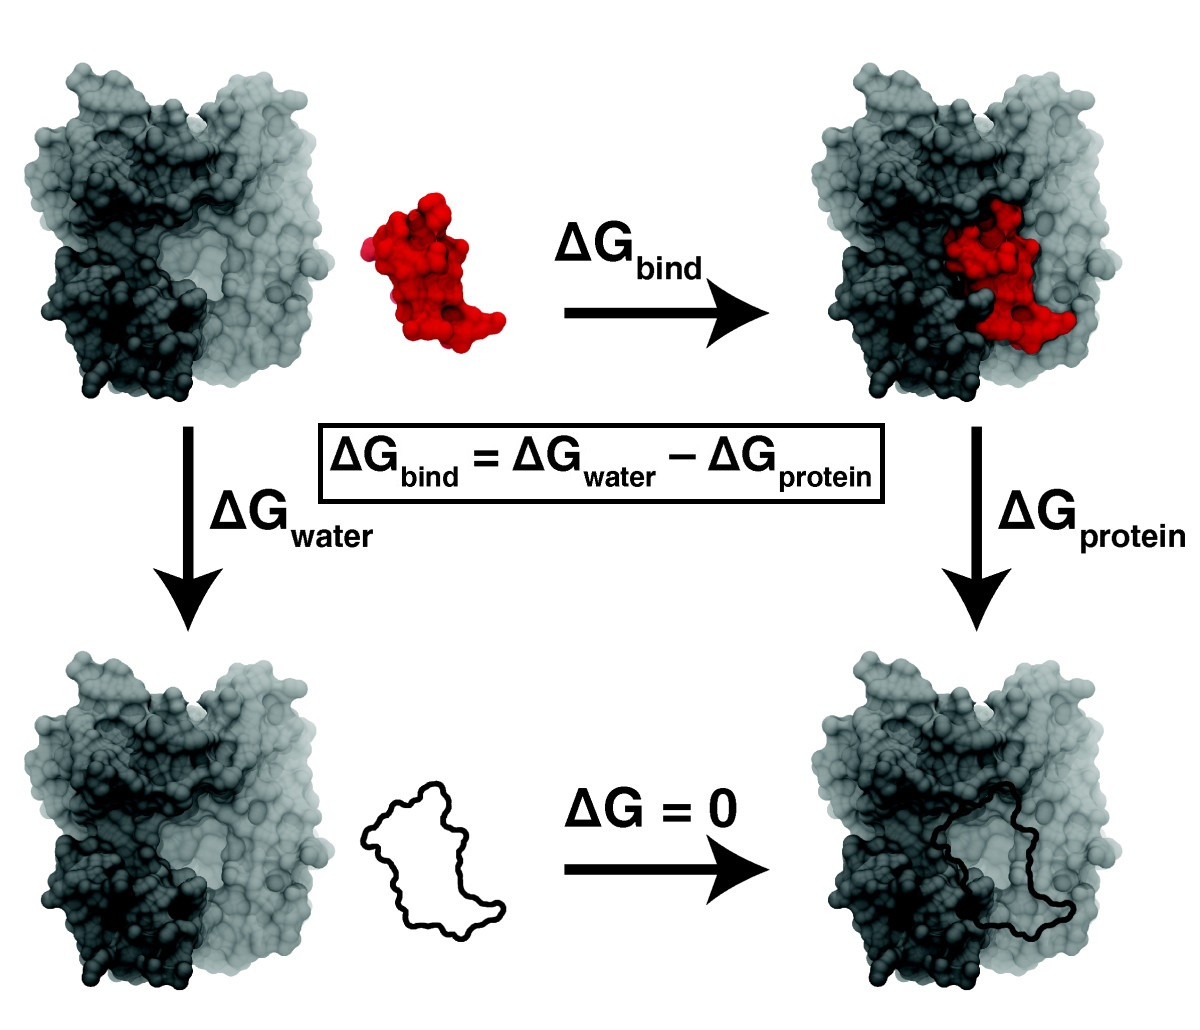
\includegraphics[scale=0.9]{thermcycle-cropped.jpg}
\caption[The thermodynamic cycle]{The thermodynamic cycle, adapted from Durrant and McCammon\cite{durrant2011molecular}}
\label{thermcycle}
\end{figure}

However, free energy is a state function, and as a result, $\Delta G_{bind}$ can be expressed as the sum of an alternate set of free energies along a different path, as illustrated in the thermodynamic cycle in figure \ref{thermcycle}. This alternate pathway involves the computation of two free energies of solvation, $\Delta G_{water}$ and $\Delta G_{protein}$, both of which depend only on small conformational changes accessible to MD, such as side chain rotations, which occur on the \si{\pico\second} to \si{\nano\second} scale\cite{harvey2012high}.

\section{Bridge sampling, the BAR estimator and beyond}
\label{barsubsec}

The problem of directly calculating $\Delta G_{bind}$ has been recast as the problem of indirectly calculating $\Delta G_{bind}$ via the thermodynamic cycle. Given a collection of sampled conformations, what remains is the second phase of free energy calculation: estimation. A wide variety of estimators exist\cite{shirts2007alchemical,pohorille2010good,christ2010basic}, but it has been shown that asymptotically, estimators derived from bridge sampling methods, notably the Bennett acceptance ratio (BAR)\cite{bennett1976efficient}, are unbiased and have the lowest variance of known estimators\cite{shirts2007alchemical,shirts2003equilibrium,shirts2008statistically}. Additionally, in empirical tests, BAR has been shown to outperform competing algorithms, specifically exponential averaging (EXP) and thermodynamic integration (TI)\cite{shirts2005comparison}.

Bridge sampling is a generalized form of BAR from the statistics literature, used for estimating ratios of normalizing constants\cite{meng2002warp,gelman1998simulating,meng1996simulating}. The bridge sampling identity is:
\begin{equation} \label{bridgesamE}
r \equiv \frac{c_1}{c_2} = \frac{E_2[q_1(w)\alpha(w)]}{E_1[q_2(w)\alpha(w)]}
\end{equation}

\noindent where $c_i$ is the normalizing constant, $\alpha(w)$ is an arbitrary function, and $E_i$ denotes the expectation with respect to $p_i$. Given a set of draws from $p_1$ and $p_2$, the ratio estimate is:
\begin{equation} \label{bridgesam}
\hat{r}=\frac{\frac{1}{n_2}\sum_{j=1}^{n_2}q_1(w_{2j})\alpha(w_{2j})}{\frac{1}{n_1}\sum_{j=1}^{n_1}q_2(w_{1j})\alpha(w_{1j})}
\end{equation}

\noindent where $\{w_{i1}, ..., w_{in}\}$ are draws from $p_i$, $i=1,2$.

Equation \eqref{bridgesam} defines the bridge sampling class of estimators for a range of $\alpha$ functions. BAR is defined by the choice of $\alpha$ as: 
\begin{equation}
\alpha ~\propto~ (s_1 q_1+s_2 r q_2)^{-1}
\end{equation}

\noindent where $s_i=n_i/(n_1+n_2)$. This $\alpha$ minimizes the asymptotic variance of $\log(\hat{r})$ as well as the asymptotic relative variance, $E(\hat{r}-r)^2/r^2$, when the draws are independent\cite{meng2002warp}. As $\alpha$ depends on the unknown ratio, iterative methods are used to estimate $r$\cite{meng1996simulating}.

From equation \eqref{bridgesamE}, it is apparent that when the phase space overlap between $p_1$ and $p_2$ is small, the variance of $\hat{r}$ will be large: the expectations are dominated by rare sampling events in the small overlap region. For macromolecules, small phase space overlap is the rule, rather than the exception\cite{wu2005phase1,wu2005phase2}. To remedy this, a series of intermediate distributions can be introduced to increase the overlap between adjacent states\cite{shirts2007alchemical}. These intermediates are termed ``alchemical intermediates," as these distributions define non-physical entities: fictitious molecules whose potential functions are defined as a mixture between those of the two real, physical endpoints. A collection of alchemical intermediates connecting two distributions of interest is called an alchemical path. The most widespread alchemical intermediate generation scheme is $\lambda$-scaling\cite{shirts2007alchemical,christ2010basic}:
\begin{equation} \label{lambdascaling}
U_{\lambda}(\boldsymbol{x}, \lambda)= (1-\lambda) U_1(\boldsymbol{x}) + \lambda U_2(\boldsymbol{x})
\end{equation}

\noindent $\lambda$ varies between 0 and 1, allowing for a range of potential functions from those defining the real systems $U_1$ or $U_2$ for $\lambda$ equals 0 and 1 respectively, to some intermediate, alchemical system when $\lambda$ takes any other value. The unnormalized density is given by:
\begin{equation}
q_\lambda(\boldsymbol{x}, \lambda) = \exp(-\beta U_\lambda(\boldsymbol{x}, \lambda))
\end{equation}

\noindent The introduction of intermediate distributions provides a way to approach ratio estimation with a divide and conquer strategy. Until the phase space overlap between adjacent states is sufficient for reliable ratio estimation, alchemical intermediates can be introduced to further improve overlap and simplify the estimation problem. The result of a single division is illustrated below:
\begin{equation} \label{tbar}
\begin{split}
\Delta G = G_2-G_1 &= (G_2-G_i) + (G_i-G_1) \\
 &= -\beta^{-1}\log(Z_2/Z_i) -\beta^{-1}\log(Z_i/Z_1) \\
 &= -\beta^{-1} \log\left(\frac{Z_2}{Z_i} * \frac{Z_i}{Z_1}\right) \\
 &= -\beta^{-1} \log\left(\frac{Z_2}{Z_1}\right)
\end{split}
\end{equation}

\noindent where $G_i$ and $Z_i$ respectively represent the free energy and partition function of an alchemical intermediate, $i$. For an arbitrary number of intermediates, the telescoping product form in the penultimate line of \eqref{tbar} remains equivalent to the desired ratio in the final line. 

\section{Alchemical intermediate selection}

Careful alchemical intermediate selection has been the focus of several research efforts in the chemical physics literature\cite{pham2011identifying,lu1999optimal,blondel2004ensemble,resat1993studies}, but a widely accepted and used method for intermediate selection is yet to emerge\cite{wu2005phase2}. For the alchemical intermediate generation scheme defined in equation \eqref{lambdascaling}, there are two fundamental choices to be made: how many alchemical intermediates to generate, and which $\lambda$ values they will take. Suggested methods for intermediate selection range from specific Gaussian quadrature rules\cite{AMBER14manual}, to loose guidelines recommending a two step process\cite{shirts2007alchemical}, to dynamic $\lambda$ variation in slow growth methods\cite{pearlman1989new}. For one dimensional path sampling, Gelman and Meng\cite{gelman1998simulating} derive an expression for the optimal prior density.

\begin{figure}
    \centering
    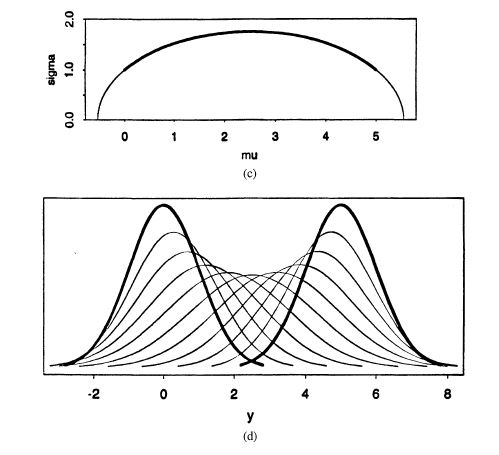
\includegraphics[scale=0.6]{pathsampling.jpg}
    \caption[Gelman and Meng's optimal bridging densities for normal distributions]{Figure from Gelman and Meng (1998). Optimal path from $\mathcal{N}(0,1)$ to $\mathcal{N}(5,1)$ in ($\mu, \sigma$) space. Top panel: Parameter representation. Bottom panel: Density representation for selected intermediates.}
    \label{GMnormnorm}
\end{figure}

In the same study, Gelman and Meng reported an even more striking result, shown in figure \ref{GMnormnorm}.
For a transition between normal distributions with continuous paths, by expanding the distribution space to allow both the mean and variance to vary, as opposed to only the mean, a new minimum variance path was found that outperformed the optimal direct one dimensional solution. For alchemical intermediate selection, multivariate representations of the potential are analogous to this expansion of the distribution space. The intermediate selection problem becomes more difficult, but with a larger potential payoff.